% Idealised directional spectrum
% Author: Marco Miani
\documentclass{article}
% Set target color model to RGB
\usepackage[rgb]{xcolor}
\usepackage{tikz}
\begin{document}
\begin{figure}[t]
	
	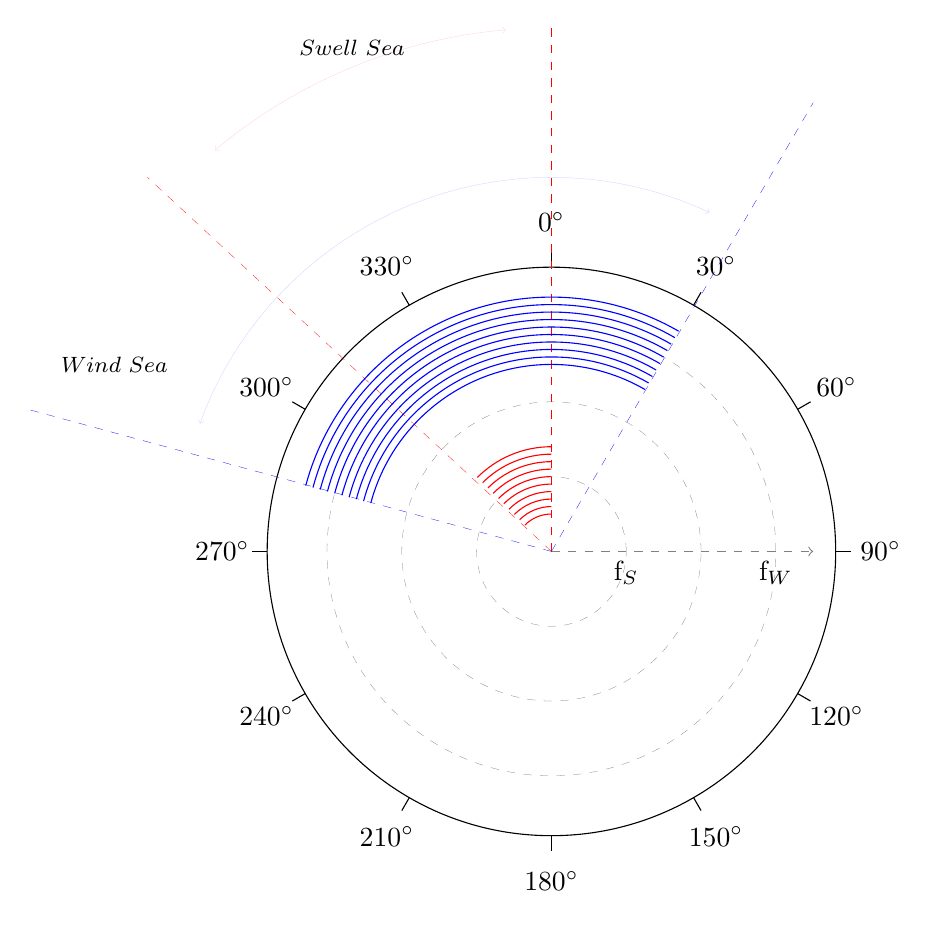
\begin{tikzpicture}[scale=.95]	
	\draw (0, 0) circle (3.8cm);
	\foreach \x  in {0, 30, ..., 330}
	\draw (-\x+90:3.8) -- (-\x+90:4.0) (-\x+90:4.4) node {$\x^\circ$};
	\foreach \x  in {0,1, ..., 3}
	\draw[dashed,ultra thin,gray] (0,0)circle(\x);
	\draw[->,dashed,gray](0,0) to[] (3.5,0);
	%Add labels with names of the primary and secondary colors.
	\foreach \x/\text in {1/f$_{S}$, 3/f$_{W}$}
	\draw (\x,0) node [below]{\text};
	\foreach \x/\text in {.5,.6,...,1.5}
	\draw [-,thin,red] (90:\x) arc(90:135:\x);
	\draw[-,ultra thin,red,dashed] (0,0) to[] (0,7);
	\draw[-,ultra thin,red,dashed] (0,0) to[] (-5.4,5);
	\foreach \x/\text in {2.5,2.6,...,3.5}
	\draw [-,thin,blue] (60:\x) arc(60:165:\x);	
	\draw[-,ultra thin,blue,dashed] (0,0) to[] (3.5,6);
	\draw[-,ultra thin,blue,dashed] (0,0) to[] (-7,1.9);
		
	\draw [<->,ultra thin,blue!20] (65:5) arc(65:160:5);
	\draw [<->,ultra thin,red!20] (95:7) arc(95:130:7);
	\path[font=\footnotesize]
	(-3.5,6.5) node[above right] {$Swell\ Sea$}
	(-5,2.5) node[left] {$Wind\ Sea$};
	%(.5,0) node[above right] {$0.1\ Hz$}
%	(3.8,.2) node[left] {$0.3\ Hz$};
%	
	
	
	\end{tikzpicture}
	\caption[Idealised directional spectrum]{Idealised representation of directional spectrum (energy units omitted) for a typical north-westerly swell, mixed with presence wind sea . Typical case of Sub Developed Sea: Swell and Wind Sea occupy two different frequency bands (denoted separately with f$_{S}$$\approx$0.1 Hz and f$_W$$\approx$0.3Hz) but still a strong local wind sea is observable. It spans over a wider area, being under direct effect of wind and therefore not having had time yet to reach spectral maturation and fully develop. Conversely, swell sea (low frequencies), is the result of spectral disintegration being confined in its typical frequency domain: evidently it has travelled long distances away from where it was originated (fetch). Assume that energy is denser for swell band.}
	\label{fig:sp2d}
\end{figure}
\end{document}
